\section{2D Transonic Flow Over an Open Cavity}\label{sec:cavity}

The first case we examine is two-dimensional transonic flow over an open cavity. This model follows work conducted by Tezaur et al.~\cite{Tezaur2016,Tezaur2017}. Flow over open cavities has been studied extensively over many decades due to its practical applications in aviation (e.g. bomb or landing gear bays) and the interesting acoustic phenomena it exhibits, namely the resonant coupling of the cavity leading edge shear layer and acoustic feedback from the cavity trailing edge.

\subsection{Full-order Model}

The computational domain is modeled as a rectangular cavity set in a flat wall, with the leftmost, rightmost, and topmost boundaries of the domain open to the atmosphere. The geometry is shown in Fig.~\ref{fig:cavityGeom}. The cavity is $L =$ 91.71 mm long, and $D =$ 45.855 mm deep ($L/D = 2.0$). The wall extends 290.8 mm (a little over three cavity lengths) both upstream and downstream of the leading and trailing edges of the cavity, respectively, for a total domain length of 673.31 mm. The upper boundary (open to air) is set 290.8 mm from the main wall. No-slip wall boundary conditions are enforced at all walls. A characteristic inlet boundary condition is enforced at the left-most domain boundary, and characteristic outlet boundary conditions are enforced at the topmost and rightmost domain boundaries. These characteristic boundaries allow acoustic waves to exit the domain with minimal reflection. The mesh is composed of 125,000 quadrilateral cells, resulting in a total number of degrees of freedom of $\numDOF =$ 500,000.

\begin{figure}
    \centering
    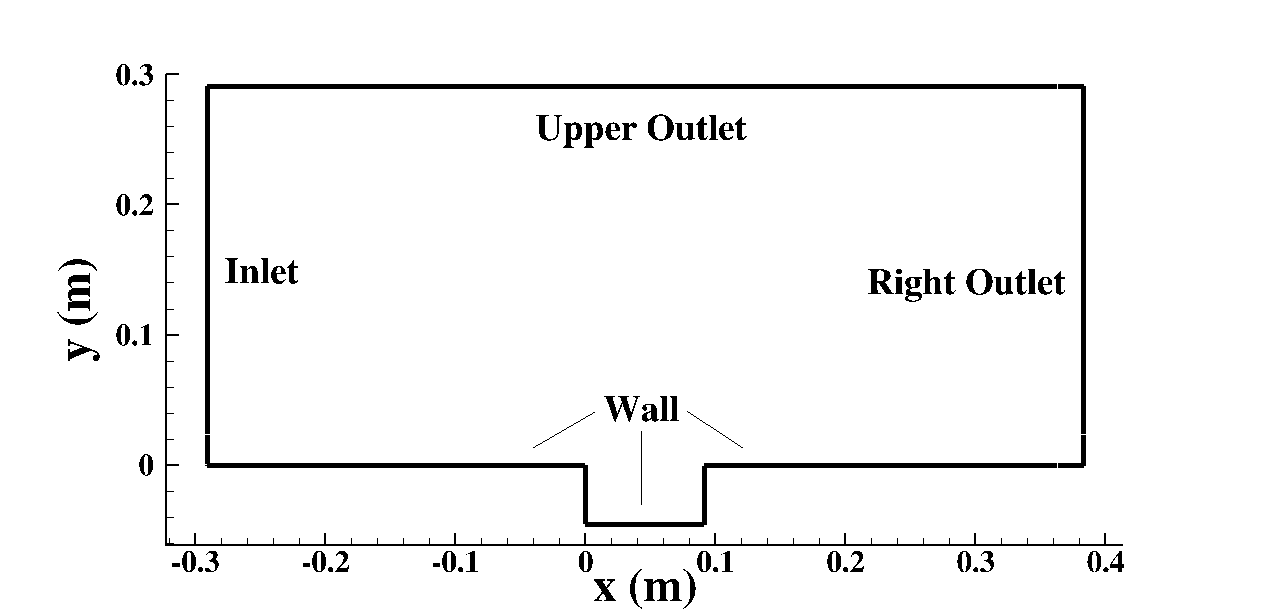
\includegraphics[width=0.9\linewidth]{Chapters/CavityAndCVRC/Images/cavity/geom.png}
    \caption{\label{fig:cavityGeom}
	2D transonic cavity flow domain.}
\end{figure}

The working gas is air, modeled as a calorically-perfect gas with the properties given in Table~\ref{tab:airProps}. The free-stream velocity is 208.7816 m/s in the +$x$-direction, the pressure is 25 Pa, and the temperature is 300 K. The working gas is air, modeled as a calorically-perfect gas (CPG) with the properties given in Table~\ref{tab:airProps}. The resulting Mach number of this flow regime is approximately 0.6, and the Reynolds number is approximately 6,500.

\begin{table}
	\centering
	\begin{tabular}{ lllll }
	\toprule
	MW (g/mol) & $c_p$ (kJ/kg-K) & $\mu$ (kg/m-s) & Pr & Sc   \\
	\midrule
	28.9604 & 1004.84 & 8.46e-7 & 0.72 & 0.62 \\
	\bottomrule
	\end{tabular}
	\caption{\label{tab:airProps}CPG properties of air for cavity flow case.}
\end{table}

The FOM is initialized with free stream conditions outside the cavity, and the inside of the cavity is initialized with free stream pressure and temperature, but zero velocity. The physical time step for the FOM simulation is $\Delta \timeVar = 1 \;\mu$s. Initial transients are allowed to dissipate and statistically-steady flow is established over 100 ms. After this point, the simulation is continued for 10 ms, during which the state is saved to disk at every physical time step, resulting in 10,001 snapshots (including the $\stateVec\left(\timeVar = 100 \; \text{ms}\right)$). All ROM simulations are restarted from $\timeVar = 100 \; \text{ms}$. Several instantaneous flow field examples are shown in Figs.~\ref{fig:cavityPressExample}-\ref{fig:cavityVExampleZoom}.

\begin{figure}
	\centering
	\ifdefined\DRAFT
		\includegraphics[width=0.9\linewidth]{example-image-a}
	\else
		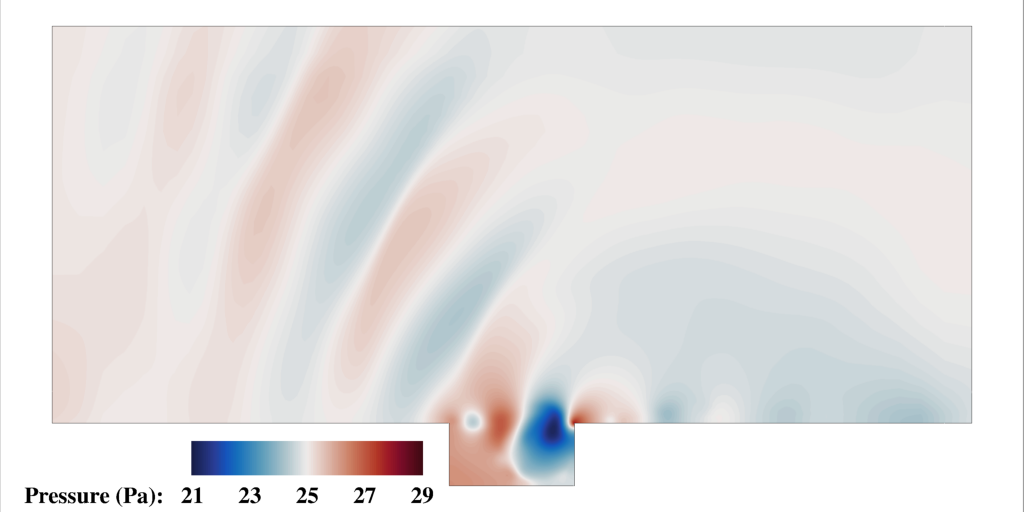
\includegraphics[width=0.9\linewidth,trim={0.5em 0.5em 0.5em 0.5em},clip]{Chapters/CavityAndCVRC/Images/cavity/pressure_example_full.png}
	\fi
	\caption{\label{fig:cavityPressExample}Pressure field at $\timeVar =$ 104 ms.}
\end{figure}

\begin{figure}
	\begin{minipage}{0.48\linewidth}
		\ifdefined\DRAFT
			\includegraphics[width=0.99\linewidth]{example-image-a}
		\else
			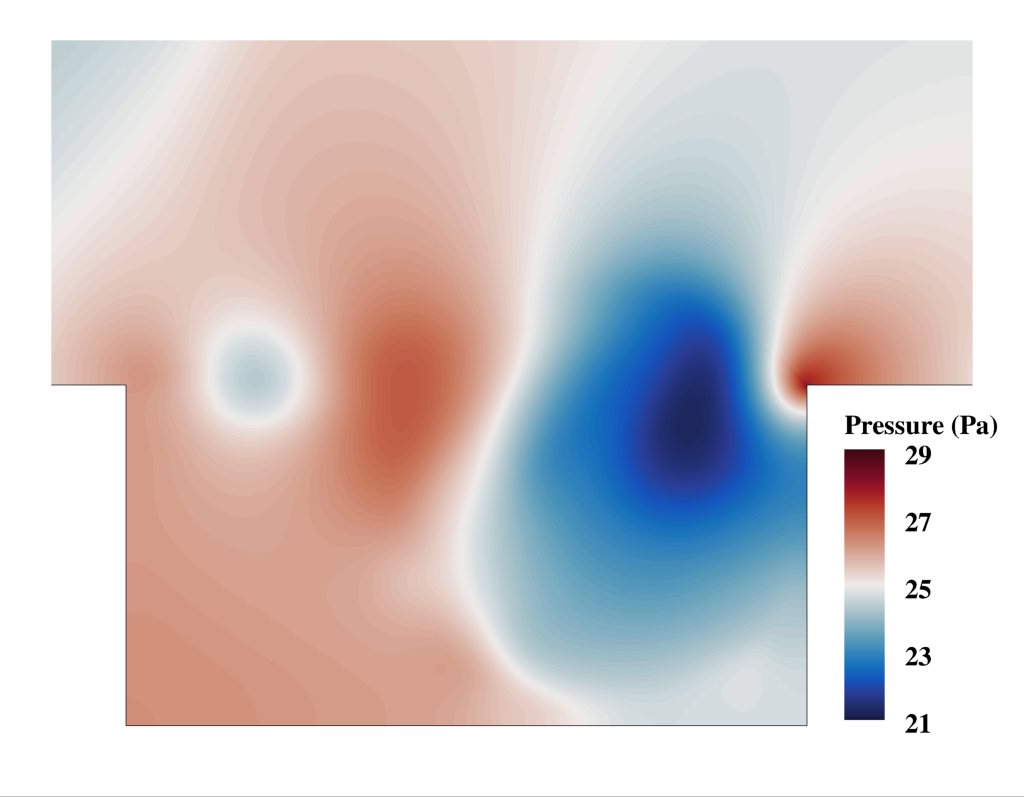
\includegraphics[width=0.99\linewidth,trim={0.5em 0.5em 0.5em 0.5em},clip]{Chapters/CavityAndCVRC/Images/cavity/pressure_example_zoom.png}
		\fi
		\caption{\label{fig:cavityPressExampleZoom}Pressure field at $\timeVar =$ 104 ms, zoomed cavity view.}
	\end{minipage} \hspace{0.5em}
	\begin{minipage}{0.48\linewidth}
		\ifdefined\DRAFT
			\includegraphics[width=0.99\linewidth]{example-image-a}
		\else
			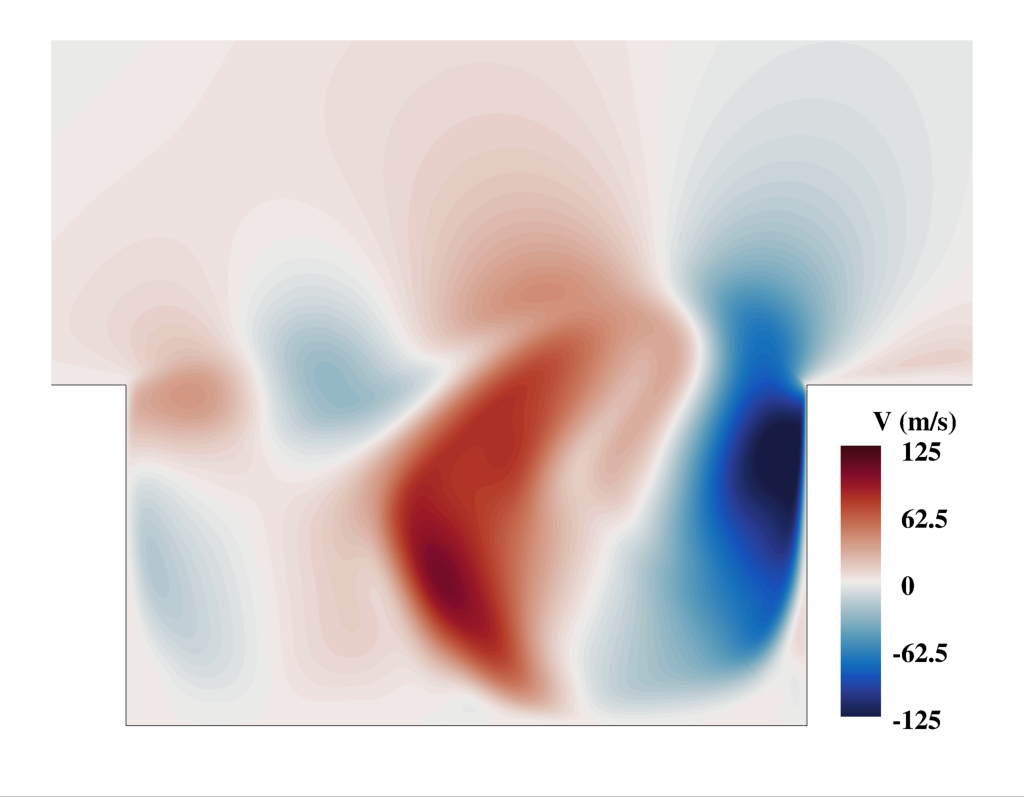
\includegraphics[width=0.99\linewidth,trim={0.5em 0.5em 0.5em 0.5em},clip]{Chapters/CavityAndCVRC/Images/cavity/y_vel_example_zoom.png}
		\fi
		\caption{\label{fig:cavityVExampleZoom}$y$-velocity field at $\timeVar =$ 104 ms, zoomed cavity view.}
	\end{minipage}
\end{figure}


The POD trial bases are computed from the 10,001 snapshots of the conservative and primitive variables. The POD energy decay is displayed in Fig.~\ref{fig:cavityPODEnergy}.

\begin{figure}
	\centering
	\ifdefined\DRAFT
		\includegraphics[width=0.8\linewidth]{example-image-a}
	\else
		\includegraphics[width=0.8\linewidth]{example-image-a}
	\fi
	\caption{\label{fig:cavityPODEnergy}POD residual energy decay for 2D cavity flow conservative and primitive state datasets.}
\end{figure}